\documentclass[12pt]{extarticle}
\usepackage[margin=1in]{geometry}
\usepackage{amssymb}
\usepackage{amsmath}
\usepackage{url}
\usepackage{bm}
\usepackage{color}
\usepackage{cancel}
\usepackage{verbatim}
\usepackage{fancyvrb}
\usepackage{datatool}
\usepackage{graphicx}

%My commands
\newcommand{\Oip}{\mathcal{O}^p_{i}}
\newcommand{\Oi}{\mathcal{O}_{i}}
\newcommand{\Oij}{\mathcal{O}_{ij}}
\newcommand{\Okl}{\mathcal{O}_{kl}}
\newcommand{\Oijp}{\mathcal{O}^p_{ij}}
\newcommand{\Oklp}{\mathcal{O}^p_{kl}}
\newcommand{\ket}[1]{\left| #1 \right>}
\newcommand{\bra}[1]{\left< #1 \right|}
\newcommand{\braket}[2]{\left< #1 | #2 \right>}
\newcommand{\ketbra}[2]{\left| #1 \right> \left< #2 \right|}
\newcommand{\taui}{\bm{\tau}_i}
\newcommand{\tauj}{\bm{\tau}_j}
\newcommand{\sigmai}{\bm{\sigma}_i}
\newcommand{\sigmaj}{\bm{\sigma}_j}
\newcommand{\rij}{\hat{r}_{ij}}
\newcommand{\sigmaia}{\sigma_{i\alpha}}
\newcommand{\sigmaib}{\sigma_{i\beta}}
\newcommand{\tauig}{\tau_{i\gamma}}
\newcommand{\sigmaja}{\sigma_{j\alpha}}
\newcommand{\sigmajb}{\sigma_{j\beta}}
\newcommand{\taujg}{\tau_{j\gamma}}
\newcommand{\tauij}{\taui \cdot \tauj}
\newcommand{\tia}{\tau_{i\alpha}}
\newcommand{\tja}{\tau_{j\alpha}}
\newcommand{\Aijt}{A^{\tau}_{i,j}}
\newcommand{\sigmaij}{\sigmai \cdot \sigmaj}
\newcommand{\mycolor}[1]{\textit{\textcolor{red}{#1}}}
\newcommand{\longsi}{s_1, \ldots, s_{i-1} , s, s_{i+1}, \ldots, s_A}
\newcommand{\longsij}{s_1, \ldots, s_{i-1} , s, s_{i+1}, \ldots, s_{j-1}, s', s_{j+1}, \ldots ,s_A}
\newcommand{\longsijkl}{s_1, \ldots, s_{i-1} , s'', s_{i+1}, \ldots, s_{j-1}, s''', s_{j+1}, \ldots ,s_A}
\newcommand{\Ot}{\mathcal{O}^\tau_{n\alpha}}
\newcommand{\Os}{\mathcal{O}^\sigma_{n}}
\newcommand{\Ost}{\mathcal{O}^{\sigma\tau}_{n\alpha}}
\newcommand{\detr}{\mathrm{det}}
\newcommand{\R}{\mathrm{\mathbf{R}}}
\newcommand{\subr}[1]{\color{blue}{#1}}
\newcommand{\red}[1]{{\color{red}{#1}}}
\newcommand{\dt}{\Delta\tau}

% sorting command
\newcommand{\sortitem}[2]{%
  \DTLnewrow{list}%
  \DTLnewdbentry{list}{label}{#1}%
  \DTLnewdbentry{list}{description}{#2}%
}

\newenvironment{sortedlist}%
{%
  \DTLifdbexists{list}{\DTLcleardb{list}}{\DTLnewdb{list}}%
}%
{%
  \DTLsort{label}{list}%
  \begin{description}%
    \DTLforeach*{list}{\theLabel=label,\theDesc=description}{%
      \item[\theLabel] \theDesc
    }%
  \end{description}% 
}

\title{Notes for Quantum/Nuclear Monte Carlo}
\author{Cody L. Petrie}

\begin{document}
\maketitle

\section*{Parameters in the Code}
\begin{sortedlist}
   \sortitem{\subr{addall(i,isum)}}{This is an interface that has many modules that all do something like isum=i. It's in nompi.f90 so it must be doing something like adding the energies from the different cpu's.}
   \sortitem{\subr{update}}{Sets valnow=valblk/wtblk, where blk stands for block, among other things.}
   \sortitem{sp(s,i)}{$=\braket{s}{s_i}$}
   \sortitem{spx(s,15,i)}{$=\bra{s}\Oip\ket{s_i}$, where $p$ goes over the 15 cartesian coordinates.}
   \sortitem{d2b(s,s',ij)}{$=\frac{\braket{\Phi}{R,\longsij}}{\braket{\Phi}{RS}}$}
   \sortitem{d2bip(s,s',s'',s''',ij,kl)}{$=\frac{\braket{\Phi}{R,s_1,\ldots,s,\ldots,s',\ldots,s'',\ldots,s''',\ldots,s_A}}{\braket{\Phi}{R,S}}$ OR}
   \sortitem{f2b(s,s',ij)}{$=\sum\limits_{p=1}^{39}f^{p}_{ij}\bra{ss'}\mathcal{O}^{p}_{ij}\ket{s_is_j}$, where $O^p_{ij} = \sigma_{i\alpha}\sigma_{j\beta}+\tau_{i\alpha}\tau_{j\alpha}+\sigma_{i\alpha}\tau_{i\gamma}\sigma_{j\beta}\tau_{j\gamma}$, 9+3+27=39 operators}
   \sortitem{fst(3,3,ij)}{$=f$ in front of specific operator}
%   \sortitem{ph(i,4,j,idet)}{$=\sum\limits_k S_{ik}\bra{k}\mathcal{O}_j\ket{s_j}$
   \sortitem{ph(i,4,j,idet)}{\red{fix}$=\sum\limits_k S_{ik}\bra{k}\mathcal{O}_j\ket{s}$, where $\ket{s}$ is in the $j^{th}$ spot.}
   \sortitem{sxz(s,i,j)}{$=\sum\limits_k S^{-1}_{jk}\braket{k}{\mathbf{r}_i,s}$}
   \sortitem{sxzi(s,i,j,iop)}{$=\sum\limits_k S'^{-1}_{jk}S'_{ki}(s)=\sum\limits_k S'^{-1}_{jk}\bra{k}\mathcal{O}^{iop}_{i}\ket{\mathbf{r}_i,s}$}
   \sortitem{sxzj(s,i,j)}{$=\sum\limits_k S''^{-1}_{jk}S''_{ki}(s)=\sum\limits_k S'^{-1}_{jk}\bra{k}\mathcal{O}^{iopjop}_{ij}\ket{\mathbf{r}_i,s}$, each $iop$ and $jop$ is looped over and added to d2b using call g2bval(d2b,sxzj,fij).}
   \sortitem{opi(s,m)}{$=\sum\limits_k S^{-1}_{mk}\bra{k}\mathcal{O}_i\ket{\mathbf{r_i},s} = \sum\limits_{s'}\mathrm{sxz(s',i,m)}\bra{s'}\mathcal{O}_i\ket{s}$}
   \sortitem{di(m)}{$=\sum\limits_k S^{-1}_{mk}\bra{k}\mathcal{O}_i\ket{\mathbf{r_i},s_i} = \sum\limits_s \mathrm{opi(s,m)}\braket{s}{s_i}$}
   \sortitem{sx15(s,15,i,j)}{$=\sum\limits_k S^{-1}_{jk}\bra{k}\sum\limits_{kop=1}^{15}\mathcal{O}_{kop}\ket{\mathbf{r},s} = \mathrm{opmult(sxz0)}$, where sx15(:,kop,:,k) = opi(s,k)}
   \sortitem{\subr{sxzupdate(sxznew(out),detrat(out),sxzold,i,opi,sp)}}{Here the outputted detrat is simply di(i).}
   \sortitem{\subr{vnpsi2(w,dopot)}}{This subroutine returns the wave function, and the potential if dopot=.true.}
   \sortitem{\subr{hspot(???)}}{???}
   \sortitem{d15(kop)}{=di(i)$=\sum\limits_k S^{-1}_{ik}\bra{k}\mathcal{O}_i\ket{\mathbf{r},s_i} = (S'/S)_{ii}$ for a specific kop (1 of 15)}
   \sortitem{\subr{opmult(sp)}}{This multiplies sp(s,i) by the 15 operators in this order 1-3 sx,sy,sz, 4-6 tx,ty,tz, 7-9 sx*(tx,ty,tz), 10-12 sy*(tx,ty,tz), 13-15 sz*(tx,ty,tz). This outputs opmult(s,kop,i)}
   \sortitem{\subr{g2bval(d2b,sxz,fij)}}{Given sxz this computes the d2b terms.}
   \sortitem{\subr{op2val(d2b,sp,spx)}}{Makes tz, sz, and stz, and makes tau, sigma, and sigtau.}
   \sortitem{tau($\alpha$,$\alpha$,ij)}{$\sum\limits_{ss'=1}^4$ d2b(s,s',ij) $\bra{ss'}\tau_{\alpha i}\tau_{\alpha j}\ket{s_is_j}$}
   \sortitem{sigma($\alpha$,$\beta$,ij)}{$\sum\limits_{ss'=1}^4$ d2b(s,s',ij) $\bra{ss'}\sigma_{\alpha i}\sigma_{\beta j}\ket{s_is_j}$}
   \sortitem{sigtau($\alpha$,$\beta$,$\gamma$,$\gamma$,ij)}{$\sum\limits_{ss'=1}^4$ d2b(s,s',ij) $\bra{ss'}\sigma_{\alpha i}\tau_{\gamma i}\sigma_{\beta j}\tau_{\gamma j}\ket{s_is_j}$}
   \sortitem{tz(s,s')}{=spx(s,$\tau_\alpha$,i)*spx(s',$\tau_\alpha$,j)$=\bra{s,s'}\tau_{\alpha i}\tau_{\alpha j}\ket{s_i s_j}$}
   \sortitem{sz(s,s')}{=spx(s,$\sigma_\alpha$,i)*spx(s',$\sigma_\beta$,j)$=\bra{s,s'}\sigma_{\alpha i}\sigma_{\beta j}\ket{s_i s_j}$}
   \sortitem{stz(s,s')}{=spx(s,$\sigma_\alpha\tau_\gamma$,i)*spx(s',$\sigma_\beta\tau_\gamma$,j)$=\bra{s,s'}\sigma_{\alpha i}\tau_{\gamma i}\sigma_{\beta j}\tau_{\gamma j}\ket{s_i s_j}$}
   \sortitem{cvs(2)}{=$\sum\limits_{\alpha=1}^3$$\sum\limits_{ss'=1}^4$ d2b(s,s',ij) $\bra{ss'} v2(i,j) \tau_{\alpha i}\tau_{\alpha j}\ket{s_is_j}$}
   \sortitem{cvs(3)}{=$\sum\limits_{\alpha=1}^3$$\sum\limits_{ss'=1}^4$ d2b(s,s',ij) $\bra{ss'}v3(i,j)\sigma_{\alpha i}\sigma_{\alpha j}\ket{s_is_j}$}
   \sortitem{cvs(4)}{=$\sum\limits_{\alpha=1}^3 \sum\limits_{\gamma=1}^3$$\sum\limits_{ss'=1}^4$ d2b(s,s',ij) $\bra{ss'}v4(i,j)\sigma_{\alpha i}\tau_{\gamma i}\sigma_{\alpha j}\tau_{\gamma j}\ket{s_is_j}$}
   \sortitem{cvs(5)}{=$\sum\limits_{\alpha=1}^3 \sum\limits_{\beta=1}^3$$\sum\limits_{ss'=1}^4$ d2b(s,s',ij) $\bra{ss'}v5(\alpha,i,\beta,j)\sigma_{\alpha i}\sigma_{\beta j}\ket{s_is_j}$}
   \sortitem{cvs(6)}{=$\sum\limits_{\alpha=1}^3 \sum\limits_{\beta=1}^3 \sum\limits_{\gamma=1}^3$$\sum\limits_{ss'=1}^4$ d2b(s,s',ij) $\bra{ss'}v6(\alpha,i,\beta,j)\sigma_{\alpha i}\tau_{\gamma i}\sigma_{\beta j}\tau_{\gamma j}\ket{s_is_j}$}
\end{sortedlist}

\section*{Variational Monte Carlo}
\textbf{Steps for Metropolis Algorithm:}
\begin{enumerate}
   \item{Start with some random walker configuration $\R$}
   \item{Propose a move to a new walker $\R'$ from the distribution $T(\R'\leftarrow\R)$}
   \item{The probability of accepting the move is given by \[A(\R'\leftarrow\R) = \mathrm{min}\left(1,\frac{T(\R'\leftarrow\R)P(\R')}{T(\R'\leftarrow\R)P(\R)}\right).\] The move is accepted if $U[0,1]<A(\R'\leftarrow\R)$.}
   \item{Repeat from step 2.}
\end{enumerate}
\textbf{Variational Energy (In terms of $E_L(\R)$ and $P(\R)$), x2 + $E_L$ and $P$:}
\begin{align*}
   E_V = \frac{\int\Psi^*(\R)\hat{H}\Psi(\R)d\R}{\int\Psi^*(\R)\Psi(\R)d\R} = \int P(\R)E_L(\R)d\R \\ P(\R) = |\Psi_T(\R)|^2/\int |\Psi_T(\R)|^2d\R\ \\ E_L(\R) = \Psi_T^{-1}(\R)\hat{H}\Psi_T(\R)
\end{align*}
\textbf{Sampled Variational Energy:}
\begin{equation*}
   E_V \approx \frac{1}{N}\sum\limits_{n=1}^N E_L(\R_n)
\end{equation*}
where $\R_n$ are drawn from $P(\R)$.

\section*{General Physics}
\textbf{Atomic Shell Model}
\begin{itemize}
   \item \textbf{Shells} are areas in which an electron can "orbit" a nucleus. They correspond to the principle quantum numbers (n=1,2,3,4,...) where n=1 is the closest shell.
   \item The number of allowed electrons is controlled by the spin statistics the other allowed quantum numbers being l=0,1,...,n-1 and ml=-l,...,l. The number allowed for each shell is all the possible times two since ms=-1/2,1/2.
   \item \textbf{Subshells} are given by the l quantum numbers where l=1,2,3,4 are s,p,d,f,g.
   \item List of how many each shell can hold
   \begin{figure}[h!]
      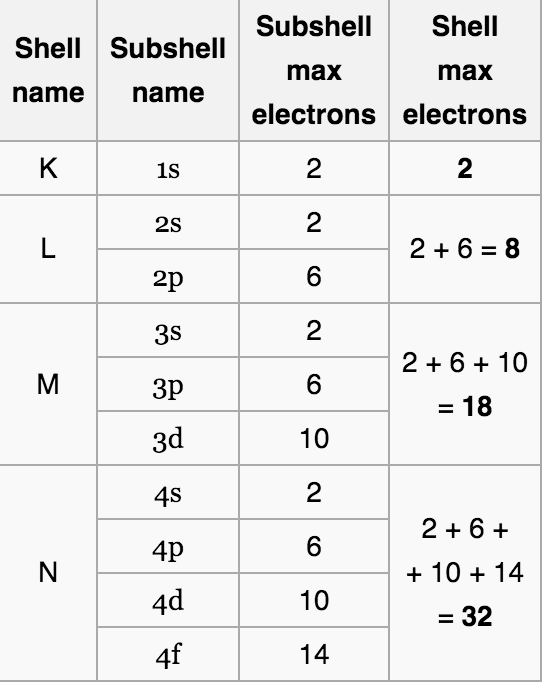
\includegraphics[width=0.25\textwidth]{shell.png}
   \end{figure}
\end{itemize}
\textbf{Nuclear Shell Model} \\
The nuclear shell model is similar to the atomic shell model except that n=1,2,3,4,... and l=0,1,2,3,... independently from n. So you can have states like 1g

\section*{Write potential as squared ops for AFDMC}
The spin-isospin dependent potential can be written in the form
\begin{equation}
   V = \sum\limits_p\sum\limits_{i<j} u^p(\rij)\Oijp.
\end{equation}
I'm going to just write this out in terms of the simplest set of terms, the $\taui\cdot\tauj$ terms.
\begin{align}
   V &= \sum\limits_{i<j} u^\tau(\rij)\Oijp \\
   &= \sum\limits_{i<j} u^\tau(\rij)\left(\tau_{ix}\tau_{jx}+\tau_{iy}\tau_{jy}+\tau_{iz}\tau_{jz}\right) \\
   &= \sum\limits_{i<j} u^\tau(\rij)\taui\cdot\tauj \\
   &= \sum\limits_\alpha\sum\limits_{i<j} u^\tau(\rij)\tia\tja.
\end{align}
These can be rewritten in terms in a martix made of of the $u$ values. In the case of the $\tau$ operators this is simple because $\Aijt=u^\tau(\rij)$. If I rewrite the potential using this, and doing a full sum over all i and j and then dividing by 2 I get
\begin{equation}
   V = \frac{1}{2}\sum\limits_{\alpha,i,j} \Aijt\tia\tja
\end{equation}
Now I want to write this matrix in terms of it's eigenvalues and eigenvectors, which are defined as
\begin{equation}
   A^{\tau}\psi_n^\tau=\lambda_n^\tau\psi_n^\tau,
\end{equation}
or if you want to write then in the matrix multiplication form
\begin{equation}
   \sum\limits_j\Aijt\psi_{n,j}^\tau = \lambda_n^\tau\psi_{n,i}^\tau.
\end{equation}
Now I want to write out the $A$ matrix in terms of it's eigenvalues and eigenvectors. I do this using eigenvector decompositon. This is defined as
\begin{equation}
   A=Q\Lambda Q^{-1},
\end{equation}
where $Q$ is the matrix of eigenvectors (so $Q_{ab}=\psi_{ab}$, the $a^{th}$ eigenvector for the $b^{th}$ particle, for example), and $\Lambda$ is the diagonal matrix of eigenvalues (so $\Lambda_{ab}=\delta_{ab}\lambda_a$). I didn't prove this, but it's roughly believable when you consider the eigenvalue equation, and doing it for each component. Also, if $Q$ is a symmetric square matrix, which it is for us, then you can write $Q^{-1}=Q^T$i. What we have in the potential is $\Aijt$, so we need to write the eigenvector decomposition in terms of the $ij^{th}$ entry. This can be done by using the definitions of matrix multiplication.
\begin{equation}
   (A\psi)_i = \sum\limits_jA_{ij}\psi_j
\end{equation}
\begin{equation}
   (AB)_{ij}=\sum\limits_\alpha A_{i\alpha} B_{\alpha j}
\end{equation}
I'll now use these two equations to get $A_{ij}$ from the definition of eigenvalue decomposition.
\begin{align}
   A_{ij} &= \left(Q\Lambda Q^T\right)_{ij} \\
   &=\sum\limits_\alpha\sum\limits_\beta Q_{i\beta}\Lambda_{\beta\alpha}Q^T_{\alpha j} \\
   &=\sum\limits_\alpha\sum\limits_\beta Q_{i\beta}\delta_{\beta\alpha}\lambda_\alpha Q^T_{\alpha j} \\
   &=\sum\limits_\alpha \lambda_\alpha Q_{i\alpha}Q^T_{\alpha j} \\
   &=\sum\limits_\alpha \lambda_\alpha \psi_{i\alpha}\psi_{j\alpha}
\end{align}
Now plug this into the equation that we had earlier for the potential to get
\begin{align}
   V &= \frac{1}{2}\sum\limits_{\alpha,i,j} \Aijt\tia\tja \\
   &= \frac{1}{2}\sum\limits_{\alpha,i,j}\sum\limits_n\lambda_n^\tau\psi_{i,n}\psi_{j,n}\tia\tja \\
   &= \frac{1}{2}\sum\limits_\alpha\sum\limits_n\left(\Ot\right)^2\lambda^\tau_n,
   \label{equ:Vtau}
\end{align}
where
\begin{equation}
   \Ot = \sum\limits_i \tau_{i\alpha}\psi^\tau_n.
\end{equation}
A similar analysis can be done for the $\Os$ and $\Ost$ operators.

\section*{Write spin-isospin dependent propagator}
The spin-isospin dependent propagator is given by
\begin{align}
   G_{SD}(R,R,\dt) = \bra{R'S'}e^{-V_{SD}\dt}\ket{RS}.
\end{align}
I'm just going to work with the $\taui\cdot\tauj$ part of the operator to make this simpler, but it could easily be expanded to include the parts including $\mathbf{\sigma}$. Using equation~\ref{equ:Vtau} I will write the propagator as
\begin{equation}
   G_{SD}(R,R,\dt) = \bra{R'S'}e^{-\frac{1}{2}\sum\limits_{\alpha,n}\left(\mathcal{O}_{n\alpha}\right)^2\lambda_n\dt}\ket{RS}.
\end{equation}
I can then pull down the sum into a product of exponentials. I am also going to combine the sum over the 3 $\alpha$ and over the $N$ $n$ into one sum over the $3N$ $n$.
\begin{equation}
   G_{SD}(R,R,\dt) = \bra{R'S'}\prod\limits_{n=1}^{3N}e^{-\frac{1}{2}\left(\mathcal{O}_\alpha\right)^2\lambda_n\dt}\ket{RS}.
\end{equation}
If I then compare this to the Hubbard-Stratanovich transformation
\begin{equation}
   e^{-\frac{1}{2}\lambda\mathcal{O}^2} = \frac{1}{\sqrt{2\pi}}\int dx e^{-x^2/2+\sqrt{-\lambda}x\mathcal{O}},
\end{equation}
and notice that $\mathcal{O}=\mathcal{O_n}$ and $\lambda=\lambda_n\dt$ and then write out an Hubbert-Stratanovich integral for each exponential in the product we get
\begin{equation}
   G_{SD}(R,R,\dt) = \prod\limits_{n=1}^{3A}\frac{1}{\sqrt{2\pi}}\int dx_n e^{-\frac{x_n^2}{2}} e^{\sqrt{-\lambda_n\dt}x_n\mathcal{O}_n}.
\end{equation}
If you expand this for all of the 15$A$ operators it just simply increases the products and you get
\begin{equation}
   G_{SD}(R,R,\dt) = \prod\limits_{n=1}^{15A}\frac{1}{\sqrt{2\pi}}\int dx_n e^{-\frac{x_n^2}{2}} e^{\sqrt{-\lambda_n\dt}x_n\mathcal{O}_n}.
\end{equation}

\section*{Uncertainty in Observables}
The thing that we calculate in the code is
\begin{equation}
   \sigma_{cal} = \sqrt{\frac{1}{N}\sum\limits_ix_i^2-\left(\frac{1}{N}\sum\limits_ix_i\right)^2}.
\end{equation}
But this gets calculated a bunch of times and so what we want is $\left<\sigma_{cal}^2\right>$. Expanding this out we get (\red{As a reference I don't completerly understand how $\left<x_1x_2\right> is \left<x\right>^2$})
\begin{align}
   \left<\sigma_{cal}^2\right> &= \left<x^2\right> - \frac{1}{N^2}\left[N\left<x^2\right>-N(N-1)\left<x\right>^2\right] \\
   &= \left<x^2\right>\left(1-\frac{1}{N}\right) - \frac{(N-1)}{N}\left<x\right>^2 \\
   &= \frac{(N-1)}{N}\left[\left<x^2\right>-\left<x\right>^2\right] \\
   &= (N-1)\frac{\sigma^2}{N}.
\end{align}
So since we want $\sigma/\sqrt{N}$ all we need to do is divide what we calculate by $\sqrt{N-1}$ and we have it.
\begin{equation}
   \frac{\sigma}{\sqrt{N}} = \sqrt{(N-1)}\sqrt{\left<\sigma_{cal}^2\right>}
\end{equation}

\section*{Definitions}
\textbf{Pedagogical:} Of or relating to teachers or education. \\
\textbf{Coherence length:} It sounds like it's something like the length over which correlations/interactions can happen. \\
\textbf{Cluster decomposition:} If a system is cluster decomposable it means that the expectation value of a product of operators (each operating in seperate regions) is equal to the product the their individual expectation values. \\
\textbf{Fock state basis:} For ferminons this is where each state is filled according to the pauli-exclusion principle. For example, with 2 particles in a three state system, with $\ket{n_{\mathbf{k1}},n_{\mathbf{k2}},n_{\mathbf{k3}}}$, you get the possible states, $\ket{110},\ket{101},\ket{011}$. \red{To me this looks right for indistinguishable particles. Is this true for distinguishable particles? For example do you need to say that 1,2,3 represent each particle and then include both states $\ket{102}$ and $\ket{201}$? In fact, when we say $\phi_1(\mathbf{r}_1)\phi_2(\mathbf{r}_2)=-\phi_1(\mathbf{r}_2)\phi_2(\mathbf{r}_1)$, are we saying that particle 1 and 2 are distinguishable?} Actually the fact that you are writing the wavefunction as an antisymmetric product means that they are indistinguishable, because any particle could be at any location. \\
\textbf{Second quantization:} The quantum states are written in a fock basis and then creation and annihilation operators are used to construct and do things with the fock states. \\
\textbf{Fermi sign problem:} Integrals involving highly oscillatory functions often do not converge. This is the case with QMC calculation involving fermions because the wave functions are antisymmetric Slater Determinants, which have positive terms with an almost identical piece with an opposite sign (oscillatory part). \\
\textbf{Path constraint:} This is a method to account for the the fermi sign problem. The overlap between the trial wave function and the walkers is complex. The path constraint method forces the walkers to stay in a region where the real part of the overlap is positive. \\
\textbf{Fixed phase approximation:} This is also a method to account for the fermi sign problem. \red{Give more explanation here.} \\
 
\end{document}
